\documentclass[14pt]{extreport}
\usepackage{gost}
\usepackage{listings}

%Тут можно вставить дополнительные пакеты

\begin{document}
	\lstset{ %
		language=Python,                % Язык программирования 
		numbers=left,                   % С какой стороны нумеровать
		basicstyle=\footnotesize,
		inputencoding=utf8,
		extendedchars=\true
	}
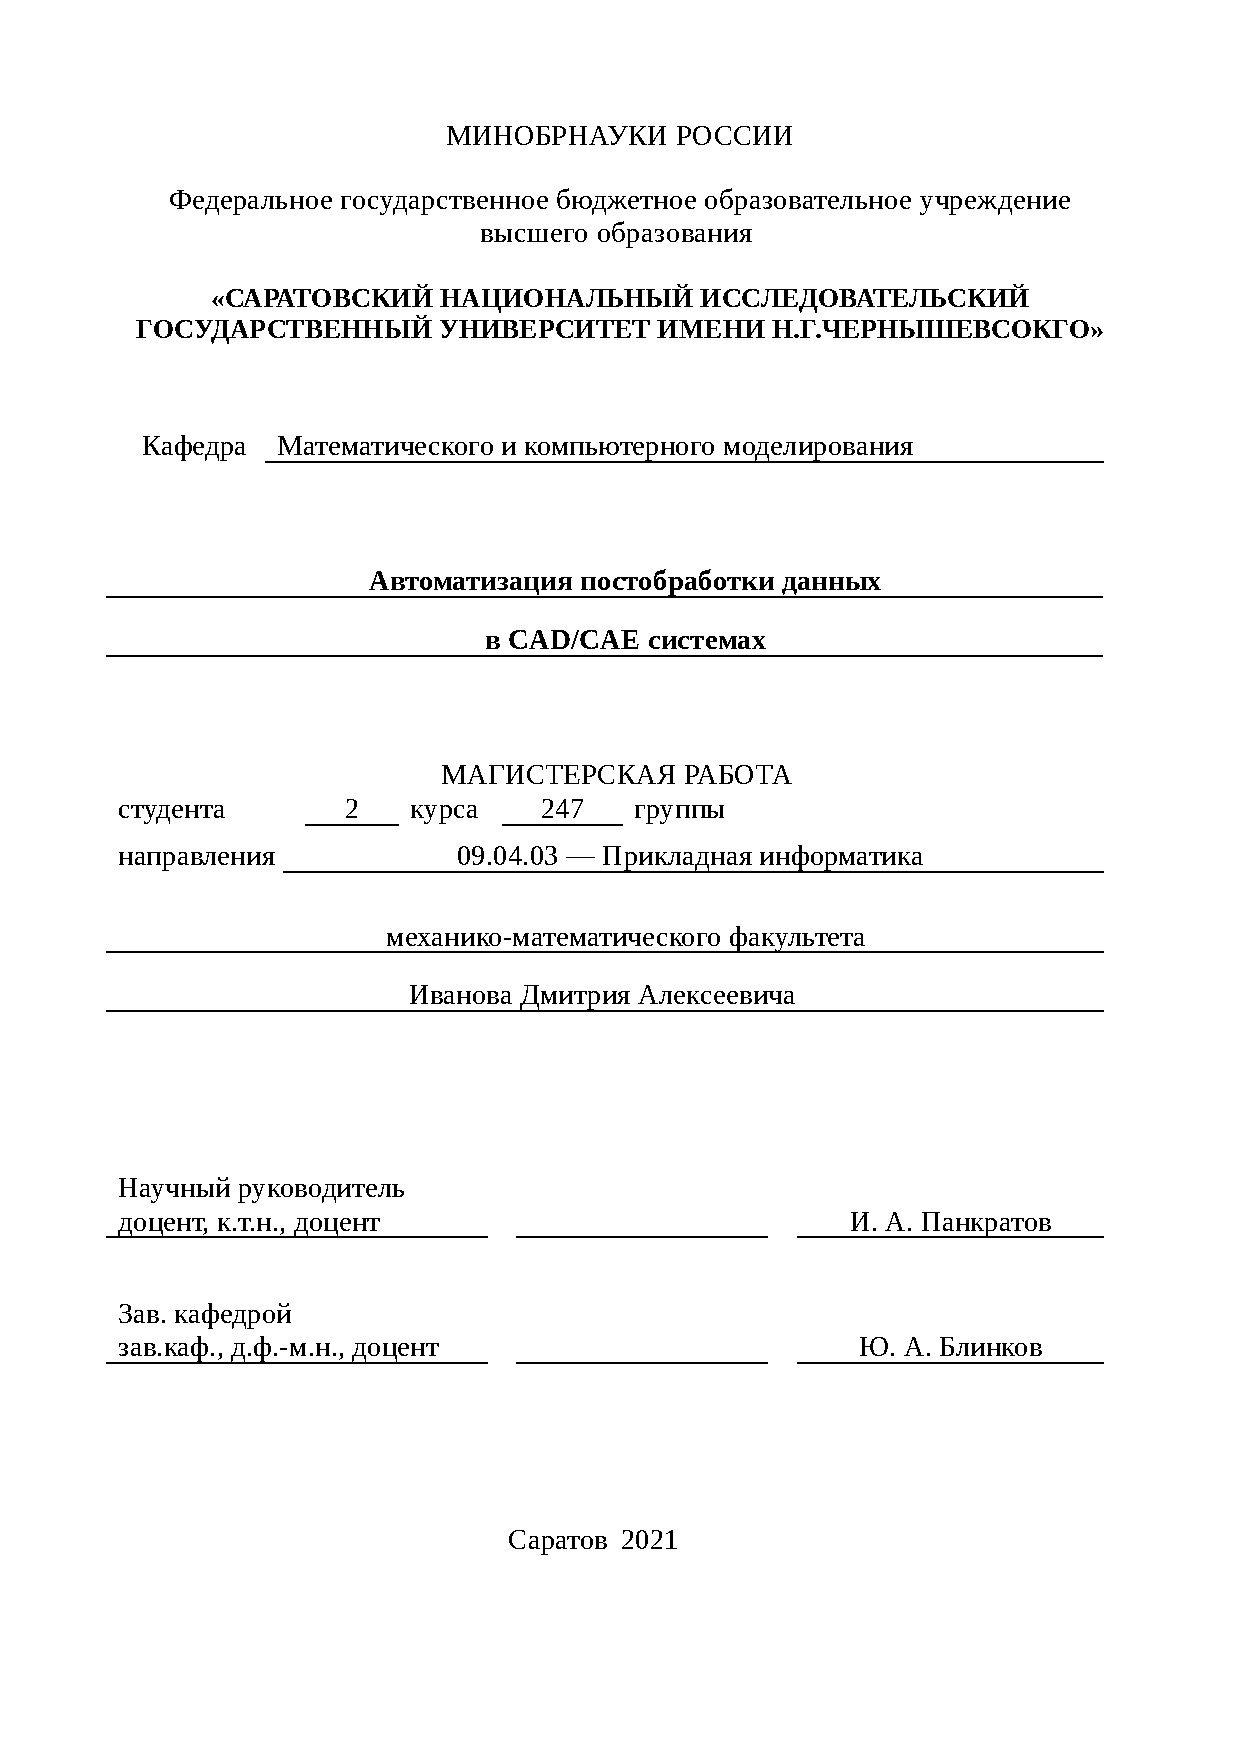
\includepdf[pages={1}]{titulCourse.pdf}

% ТЕМА: Анализ экспериментальных данных с помощью NoSQL

\tableofcontents

\intro

При обработке экспериментальных данных, полученных в результате математического моделирования физических процессов в CAD/CAE системах, особенно, когда проводиться, например, серия экспериментов, в которых входные данные незначительно изменяются часто порождается большой объем результатов, надлежащих анализу или иными словами -- пост-обработке. Причем, зачастую для анализа с полученными мало различающимися данным необходимо провести однотипные манипуляции. Учитывая все вышесказанное, становится ясна необходимость автоматизации такого процесса пост-обработки данных. 

В магистерской работе будет спроектирована и разработана информационная система позволяющая упростить процесс анализа полученных экспериментальных данных. Для автоматизации будет использован язык программирования Python, для хранения результатов -- NoSQL подход, а конкретно СУБД MongoDB. 

Таким образом целью данной курсовой работы является проектирование и разработка информационной системы, автоматизирующей рутинные операции анализа экспериментальных данных.
Задачи:
\begin{itemize}
\item Кратко рассмотреть CAD/CAE систему -- OpenFOAM и ParaView.
\item Рассмотреть существующие решения по данной тематике.
\item Спроектировать информационную систему и создать UML-диаграммы для ее описания.
\item Обзор средств разработки.
\item Разработать информационную систему.
\end{itemize}

\chapter{Краткая информация об OpenFOAM и ParaView}
\section{OpenFOAM}
OpenFOAM (англ. Open Source Field Operation And Manipulation CFD ToolBox) — открытая интегрируемая платформа для численного моделирования задач механики сплошных сред. ~\cite{OpenfoamWiki}

Это пакет программ распространяемых свободно под лицензией GNU GPL, позволяющей решать задачи механики сплошных сред, в частности: 
\begin{itemize}
\item Прочностные расчеты;
\item Гидродинамика ньютоновских и неньютоновских вязких жидкостей как в несжимаемом, \item так и сжимаемом приближении с учётом конвективного теплообмена и действием сил гравитации. Для моделирования турбулентных течений возможно использование RANS-моделей, LES- и DNS-методов. Возможно решение дозвуковых, околозвуковых и сверхзвуковых задач;
Задачи теплопроводности в твёрдом теле;
\item Многофазные задачи, в том числе с описанием химических реакций компонент потока;
\item Задачи, связанные с деформацией расчётной сетки;
\item Сопряжённые задачи;
\item Некоторые другие задачи, при математической постановке которых требуется решение дифференциальных уравнений в частных производных в условиях сложной геометрии среды;
\end{itemize}

В основе кода лежит набор библиотек, предоставляющих инструменты для решения систем дифференциальных уравнений в частных производных как в пространстве, так и во времени. Рабочим языком кода является C++. OpenFOAM состоит из приблизительно 250 программ основанных на более чем 100 библиотеках. Каждое приложения выполняет свою конкретную задачу в рамках процесса расчета. Этапы работы представленные в соответствии с рисунком ~\ref{fig1}.

\begin{figure}[H]
\centerline{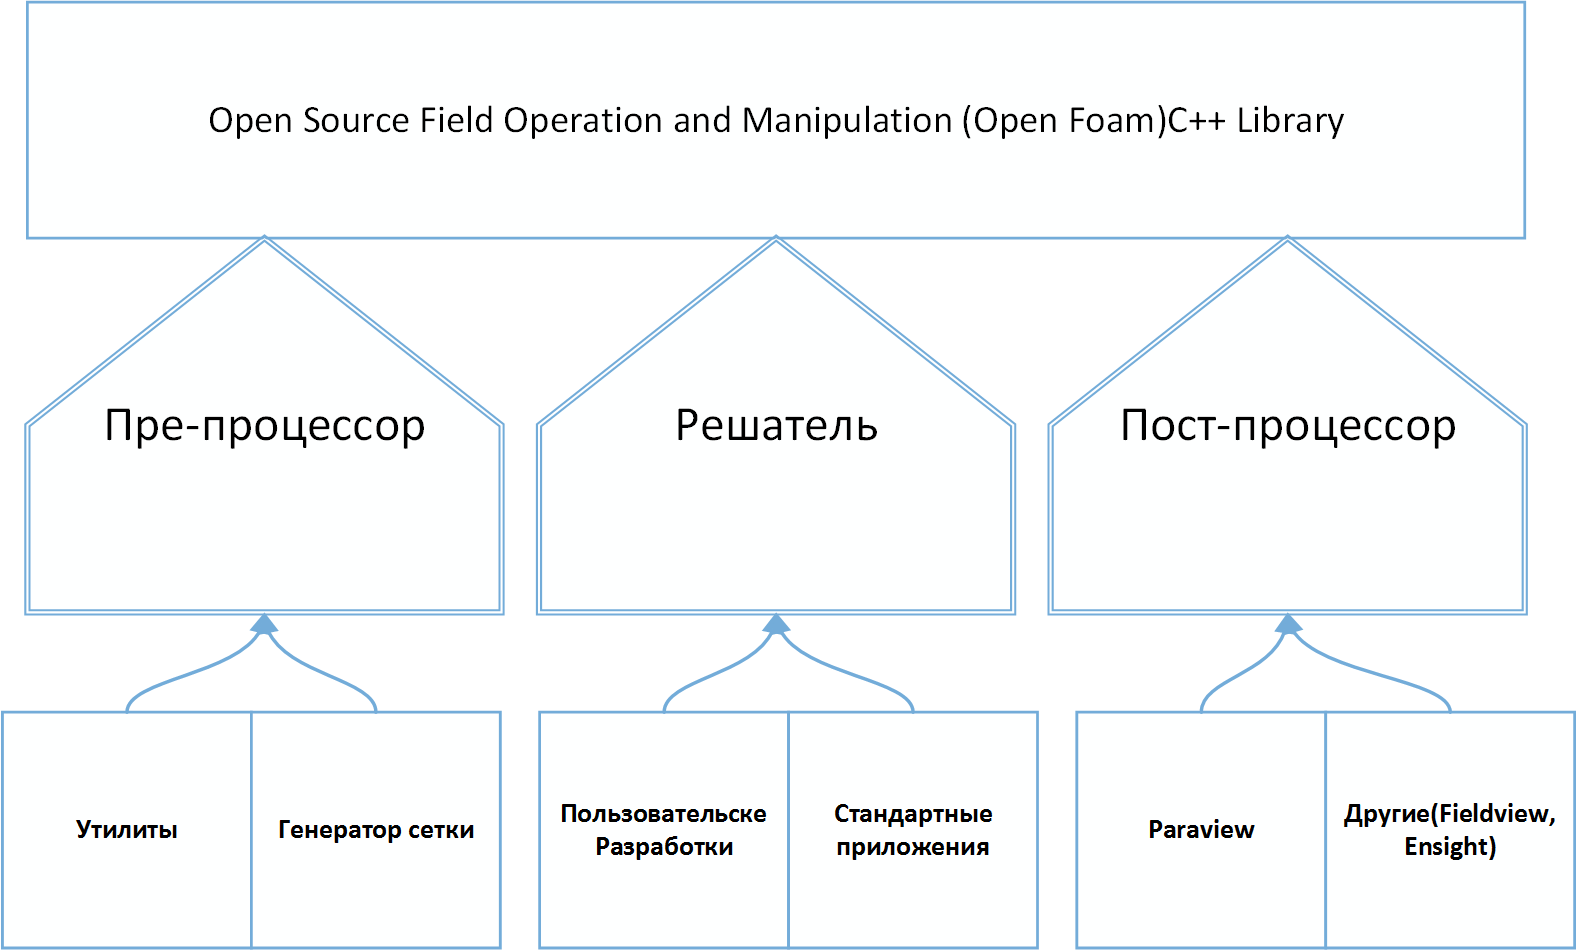
\includegraphics[width=1.0\linewidth]{OFScheme}}
\caption{Утилиты и программы входящие в пакет OpenFOAM, сгруппированные по этапам работы с расчетом}
\label{fig1}
\end{figure}

Работа с программой делится на три этапа:
\begin{enumerate}
\item Пре-процессинг;
\item Решение;
\item Пост-процессинг.
\end{enumerate}

На этапе пре-процессинга в специальных файлах задаются входные данные для рассчета примера, такие как: начальное время, конечное время, шаг и так далее. Также параметры для хранения решения: время, формат, тип сжатия. Также в препроцессинг включены настройки выбора различных схем рассчета, котоыре влияют на точность и стабильность решения. После этого отдельно генерируется расчетная область (сетка), которая впоследствии может быть обработана различными утилитами ~\cite{OpenfoamUserGuide}. Затем запускается решатель, который производит расчет. На этапе пост-процессинга полученные данные представляются в виде графиков. Также используются некоторые утилиты, например для конвертации из внутреннего формата OpenFOAM в широко используемый формат vtk.

\section{ParaView}
ParaView -- открытый графический кросс-платформенный пакет для интерактивной визуализации в исследовательских целях, разрабатываемый Национальной Лабораторией Сандиа, компанией Kitware и Национальной Лабораторией Лос-Аламоса \cite{ParaviewAbout}.

Пакет ParaView предоставляет пользователю возможности интерактивной визуализации и исследования больших массивов данных для качественного и количественного анализа.

Пакет может быть использован на компьютерах с операционными системами Windows, Linux, Mac OS X.

При разработке авторы придерживаются следующих целей:
\begin{itemize}
\item Открытость, кросс-платформенность — в пакете используются только открытые, мульти-платформенные технологии для визуализации данных.
\item Поддержка различных, в том числе, гетерогенных вычислительных систем.
\item Создание гибкого, интуитивного пользовательского интерфейса.
\end{itemize}

Таким образом, пакет ParaView во многом является скорее технологией обработки, чем всего лишь программным средством ~\cite{ParaviewWiki}.

Некоторые возможности пакета:
\begin{itemize}
\item Визуализация расчетных областей.
\item Визуализация полей (давление, скорость, температура, смещения и прочее).
\item Построение срезов областей как плоскостью, так и заданной функцией.
\item Построение изо-поверхностей.
\item Построение векторных полей и линий тока.
\item Позволяет показывать динамику развития протекающего процесса, отображая анимацию. 
\end{itemize}

Основной формат данных ParaView -- VTK, но пакет также содержит драйверы для работы с форматом OpenFOAM и поставляется вместе с дистрибутивом пакета. 

Работа с ParaView может осуществляться как в интерактивном, так и пакетном режиме.

ParaView также предлагает богатый и мощный програмный интерфейс на языке Python. Это позволяет пользователям автоматизировать обработку своих данных и использовать возможности, так называемого, набора инструментов визуализации -- Visualization Tool Kit (VTK) ~\cite{ParaviewAndPython}.

\chapter{Обзор существующих решений}
Рассматриваемая в данной курсовой работе информационная система должна выполнять пост-обработку данных, полученных в результате численно эксперимента в пакете OpenFOAM, делая упор на автоматизацию функций для работы с серией данных. Рассмотрим доступные приложение осуществляющие автоматизацию рутинных функций в рамках пакета OpenFOAM.
\section{HELYX OS}
HELYX-OS - это графический пользовательский интерфейс с открытым исходным кодом, разработанный компанией ENGYS для работы со стандартными библиотеками OpenFOAM, предоставляемыми OpenFOAM Foundation и ESI-OpenCFD. Приложение предназначено для академического использования и работы с CFD начального уровня. Распространяется в соответствии с GNU General Public License ~\cite{Helyx}.

HELYX-OS предоставляет полностью интерактивную, простую в использовании среду для выполнения всех задач предварительной обработки в процессе CFD, включая создание сетки, определение случая и выполнение решателя.

Существует также версия для корпоративного использования -- CFD HELYX.

Преимущества: 
\begin{itemize}
\item Встроенная поддержка как OpenFOAM, так и OpenFOAM+: возможность загружать существующие примеры, читая настройки непосредственно из доступных текстовых файлов проекта.
\item Программа доступна на платформах Linux и Windows. Однако версия для Windows платна.
\item Управление утилитой построения сеток snappyHexMesh, включая такие возможности как отображение геометрии и непосредственное построение прямо в окне приложения.
\item Отдельный мониторинг решателя с отслеживанием остатков решения.
\end{itemize}

В корпоративной версии также следует выделить:
\begin{itemize}
\item Высокая масштабируемость.
\item Возможность работы с использованием облачных технологий.
\item Модульность. Возможно расширение в рамках HELYX ADD-ONS, 
\end{itemize}

В соответствии с рисунком ~\ref{fig2} изображен рабочий экран программы.

\begin{figure}[H]
\centerline{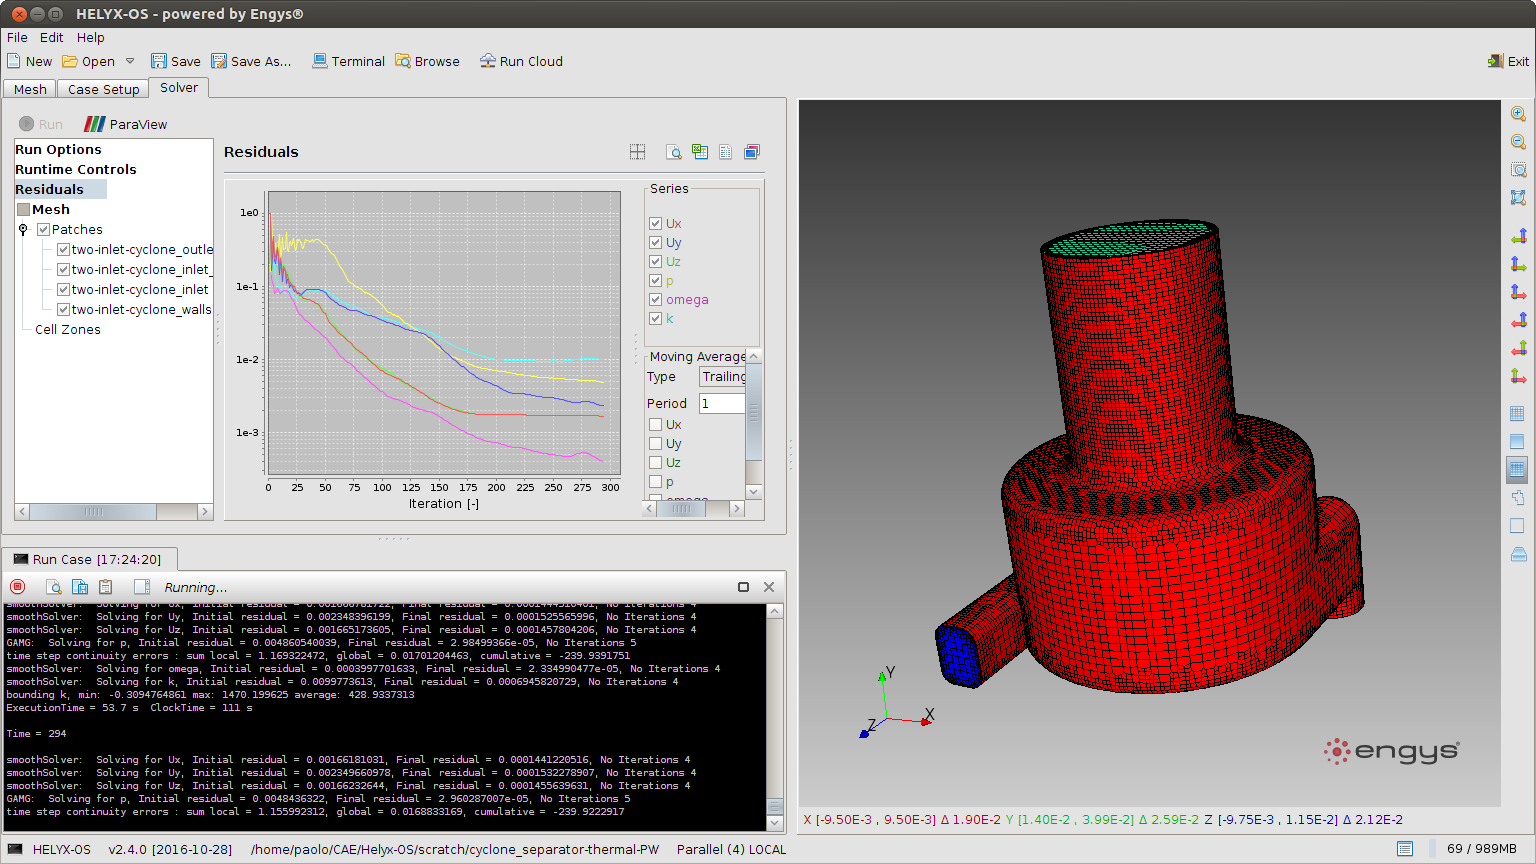
\includegraphics[width=1.0\linewidth]{helyxos}}
\caption{Рабочий экран приложения Helyx OS}
\label{fig2}
\end{figure}

\section{ANSA}
ANSA - это инструмент пре-процессинга CAE, который предоставляет все необходимые функциональные возможности для построения полной модели, от CAD-данных  до готового к вводу файла решателя, в единой интегрированной среде ~\cite{Ansa}.

Все функции программного обеспечения размещены в интегрированной среде с настраиваемым графическим интерфейсом. Программное обеспечение доступно для всех современных популярных операционных систем в 32-битной и 64-битной архитектуре с использованием многоядерных процессоров. 

Преимущества: 
\begin{itemize}
\item Эффективная обработка данных для сложных структур моделей.
\item Быстрое и качественное моделирование сложных геометрических моделей.
\item Возможность взаимодействия между моделями, созданными для разных решателей.
\item Высокоавтоматизированные процессы и инструменты настройки модели в одной программе.
\item Уменьшены зависящие от пользователя подверженные ошибкам операции.
\item Полное построение модели для многочисленных решателей в одной среде.
\end{itemize}
Рабочий экран приложения представлен в соответствии с рисунком ~\ref{fig3}.

\begin{figure}[H]
\centerline{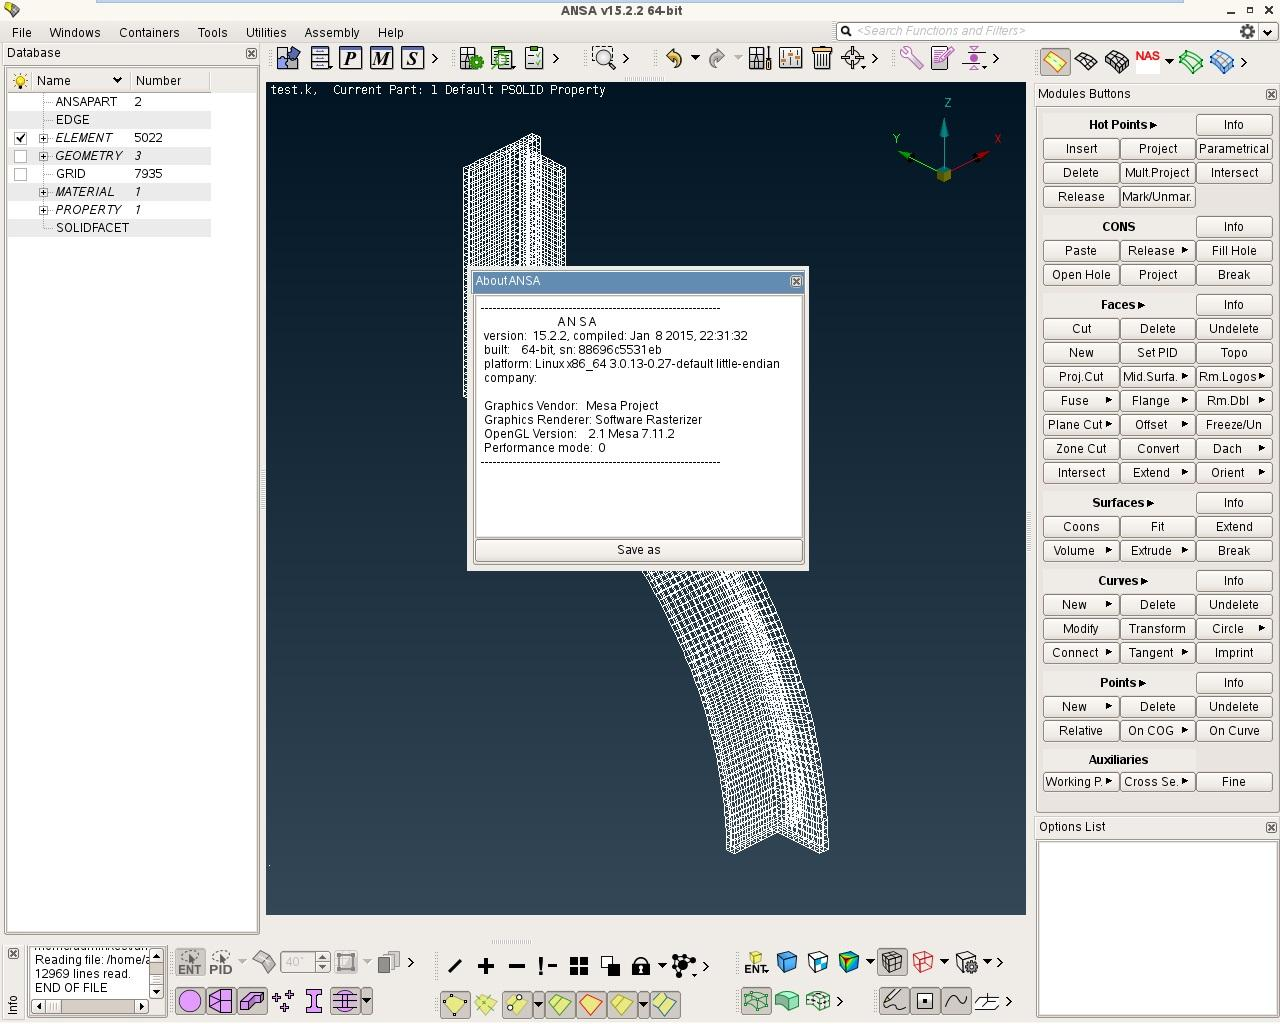
\includegraphics[width=1.0\linewidth]{ansa}}
\caption{Рабочий экран приложения ANSA}
\label{fig3}
\end{figure}

\section{CastNet}

CastNet упрощает использование технологических решений CAE для решателей с открытым исходным кодом: кроме типичного редактирования текстовых файлов, предоставляется альтернативный способ работы с OpenFOAM на основе графического интерфейса, сохраняя полную совместимость со стандартными выпусками OpenFOAM. В результате рабочий процесс становится достаточно гибким, и пользователь может в любой момент переключаться между настройкой рабочего примера на основе текстового файла и графического интерфейса пользователя.

Вид рабочего экрана приложения представлен в соответствии с рисунком ~\ref{fig4}
\begin{figure}[H]
\centerline{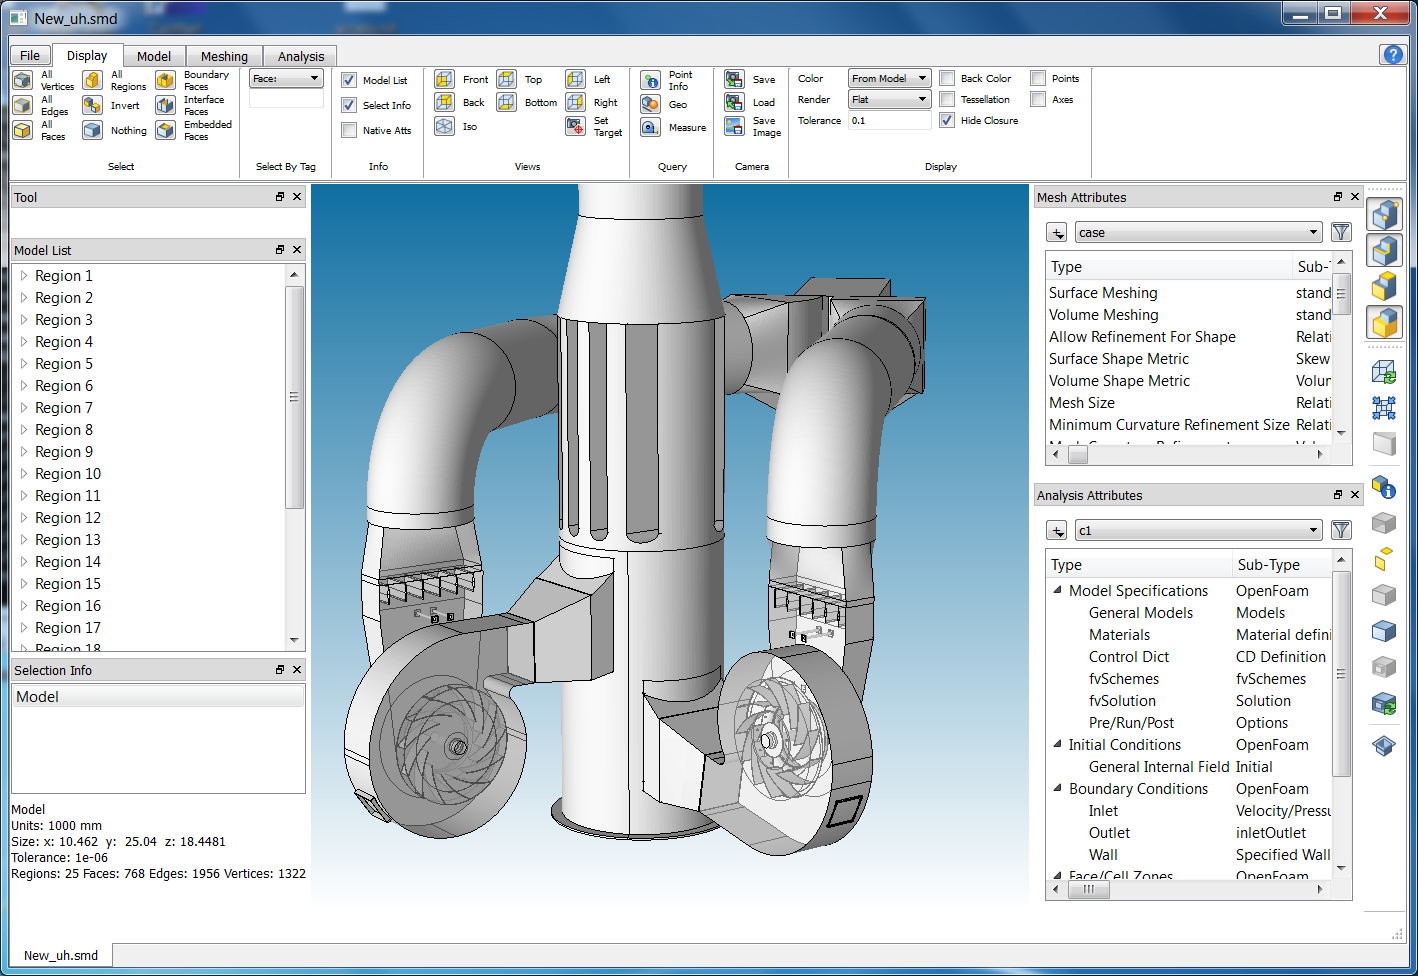
\includegraphics[width=1.0\linewidth]{castnet}}
\caption{Рабочий экран приложения CastNet}
\label{fig4}
\end{figure}

Ключевые особенности CastNet:
\begin{itemize}
\item Среда разработки на основе графического интерфейса пользователя, включающая предварительную обработку (создание сетки, настройку примера), мониторинг решения и последующую обработку. Таким образом: доступ к мощным функциям решателя с открытым исходным кодом без редактирования текстовых файлов или необходимости детального изучения структуры ключевых слов OpenFOAM.
\item Кроссплатформенное использование: поддержка среды для пакета программ OpenFOAM в операционных системах Windows и Linux.
\item Библиотека шаблонов позволяет настраивать пример для более чем 30 решателей.
\item Больше надежности в отношении результатов моделирования благодаря контролю сходимости.
\end{itemize}

\section{Итог}

Таким образом, рассмотренные существующие решения предлагают разнообразные и гибкие возможности по работе с примерами, однако ни одно из них не предоставляет функциональности по работе сразу с группой примеров, что в свою очередь вызывает трудности при анализе экспериментальных данных, которые состоят из набора примеров.  

\chapter{Проектирование информационной системы}
\section{Постановка задачи}
Необходимо спроектировать приложение, которое бы выполняло процесс пост-обработки, то есть строило графики используя экспериментальные данные полученные из пакета программ OpenFOAM. Приложение должно также работать с группами экспериментальных данных, то есть выполнять конкретное действие построения графика, например срез, с группой из разных мало отличающихся примеров. Программа должна хранить экспериментальные данные и историю операций примера, также должна быть реализована возможность экспорта графиков в файлы.
Для более подробного понимания информационной системы были построены UML-диаграммы. 

\section{Диаграмма прецедентов}
Прецеденты -- это технология определения функциональных требований к системе ~\cite{umlDistilled}. 
Диаграмма прецедентов (use case diagram) предназначена для описания взаимодействия проектируемой системы с любыми внешними или внутренними объектами - пользователями, другими системами и тому подобное.
Основными понятиями при работе с диаграммой вариантов использования являются 
Актор (Actor) -- это роль, которую выполняет пользователь или другая система, при взаимодействии с проектируемой системой.
Вариант использования -- это конечная единица взаимодействия актора и системы. 

Диаграмма вариантов использования представлена в соответствии с рисунком ~\ref{fig5}
\begin{figure}[H]
\centerline{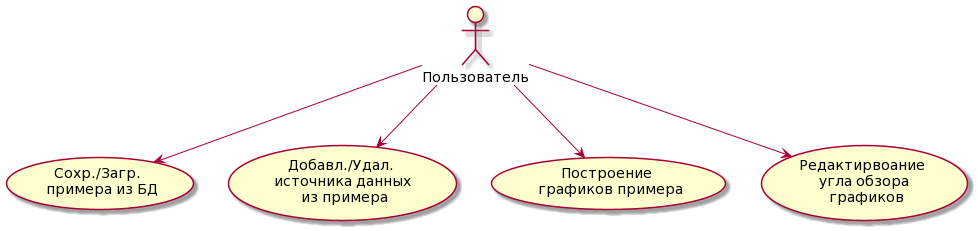
\includegraphics[width=1.0\linewidth]{userCaseDiagram}}
\caption{Диаграмма прецедентов}
\label{fig5}
\end{figure}

В соответствии с рисунком ~\ref{fig5} представлена базовая функциональность проектируемой программы. Пример или основная сущность программы состоит из списка источников данных. Каждый источник данных -- это результат конкретного численного эксперимента. Таким образом достигается цель -- работа сразу с несколькими источниками данных.   

В случае описанной программы, встречаются следующие прецеденты:
\begin{itemize}
	\item Сохранение и загрузка примера из базы данных. Работа с программой строится вокруг анализа расчетов полученных от пакета программ OpenFOAM, конфигурации данных должны сохраняться в базе данных для обеспечения сохранности информации и быстрого доступа к ней, при возрастающим объеме примеров. 
	\item Добавление и удаление источника данных из примера. Также необходимая функция для возможности быстрой и гибкой настройки примеров для получения различных срезов и углов обзора графиков.
	\item Редактирование угла обзора графиков -- изменение положения камеры в соответствии с необходимостью анализа данных.
	\item Редактирования срезов графика -- получение срезов графика для анализа экспериментальных данных.
	\item Построение графиков примера -- получение изображение в соответствии с описанными выше настройками примера.
\end{itemize}

\section{Диаграмма классов}
Диаграмма классов описывает типы объектов системы и различного рода статические отношения, которые существуют между ними. На диаграммах классов отображаются также свойства классов, операции классов и ограничения, которые накладываются на связи между объектами ~\cite{umlDistilled}.

Для удобства рассмотрения разобьем диаграмму классов на три рисунка. Каждый из которых соответствует определенной решаемой задачи. 

\subsection{Диаграмма, представляющая способ организации экспериментальных данных}

В соответствии с рисунком ~\ref{fig6} представленная диаграмма классов, иллюстрирует способ организации экспериментальных данных в приложении. 

Класс Data -- ООП представление данных полученных в результате численного эксперимента в OpenFOAM. Он неразрывно связан с классом-оберткой ExpData -- в нем экземпляру присваивается идентификатор и хранится другая служебная информация необходимая программе. 

\begin{figure}[H]
\centerline{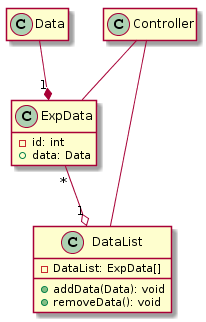
\includegraphics[height=1.0\linewidth]{classDiagram_Data-Controller}}
\caption{Диаграмма классов, представляющая способ организации экспериментальных данных}
\label{fig6}
\end{figure}

Так как проектируемое приложение должно работать с некоторым набором экспериментальных данных, то бы введен класс DataList, который, как видно в соответствии с рисунком ~\ref{fig6}, содержит список этих данных. Данный класс вступает в качестве поля класса Сase. Это класс, содержащий основную информацию о текущей сессии приложения, будет рассмотрен чуть более подробнее далее. 

Класс ExpData и DataList ассоциирован с классом Controller, где происходит их инстанцирование и инициализация. Класс Controller объединяет работу частей модели программы и связывает их с графическим интерфейсом пользователя. 

\subsection{Диаграмма для работы с базой данных и чтения экспериментальных данных}
В соответствии с рисунком ~\ref{fig7} представленная диаграмма классов, иллюстрирует работу приложения с базой данных и чтение экспериментальных данных.

Статический класс ApplicationUtils реализует чтение экспериментальных данных и настроек приложения из файла. Класс DTO (Data Transfer Object) используется в качестве промежуточной сущности для валидации данных.

Класс Database -- используется для установления соединения и работы с базой данных. Данный класс будет реализован при помощи паттерна проектирования синглтон (Singleton). Данный паттерн гарантирует, что у класса есть только один экземпляр, и предоставляет к нему глобальную точку доступа ~\cite{oop}. Такой подход дает позволяет только один раз при первом обращении произвести ресурсоемкую операцию установления соединения с базой данных, а после каждый раз при последующих обращениях возвращать уже созданный экземпляр класса. Получение различных сущностей из базы данных будет осуществляться при помощи класса DAO (Data Access Object). Этот прием позволит не передавать лишнюю информацию в модель приложения.

\begin{figure}[H]
\centerline{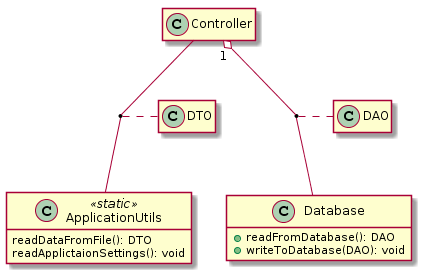
\includegraphics[width=1.0 \linewidth]{classDiagram_DB-AppUtils-Controller}}
\caption{Диаграмма классов для работы с базой данных и чтения экспериментальных данных}
\label{fig7}
\end{figure}

\subsection{Диаграмма классов для выполнения операций над графиками}
В соответствии с рисунком ~\ref{fig8} представленная диаграмма классов иллюстрирует организацию классов, реализующих операции над графиками.

Класс Case хранит необходимую информацию о текущей сессии, в частности загруженные источники данных (класс ExpData) и историю операций -- построенные графики. В классе OperationHistory непосредственно хранится информация о построенных графиках. 

\begin{figure}[H]
\centerline{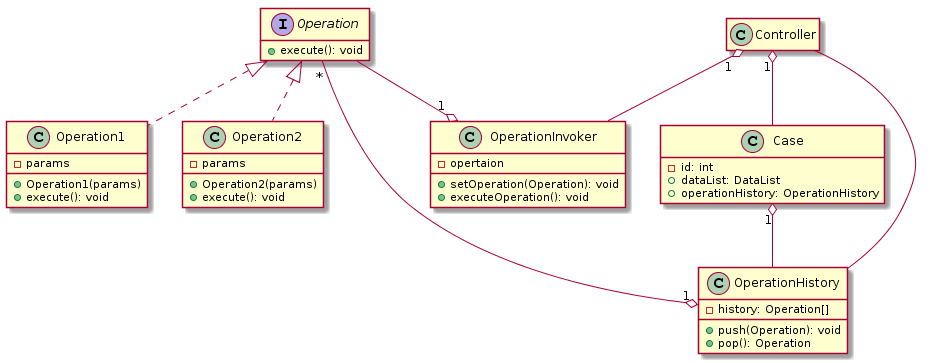
\includegraphics[width=1.1 \linewidth]{classDiagram_Case-Operaion-Controller}}
\caption{Диаграмма классов для выполнения операций над графиками}
\label{fig8}
\end{figure}

В целом, существуют разные виды графиков, а пользователем может быть последовательно запланировано несколько различных операций поэтому представляется разумным для организации этой функциональности применить паттерн проектирования команда (command или action).

Команда -- это поведенческий паттерн проектирования, который превращает запросы в объекты, позволяя передавать их как аргументы при вызове методов, ставить запросы в очередь, логировать их, а также поддерживать отмену операций \cite{pattern}. В случае данной информационной системы в роли команды выступает операция построения графика или иная связанная с этим операция.

Структура паттерна следующая: 
\begin{itemize}
\item Класс OperationInvoker хранит ссылку на объект операции и обращается к нему, когда нужно выполнить какое-то действие. OperationInvoker работает с операциями только через их общий интерфейс. Он не знает, какую конкретно опрециб использует, так как получает готовый объект операции от класса Controller.

\item Operation описывает общий для всех конкретных операций интерфейс. Здесь задан метод execute для запуска операции.

\item Конкретные операции, это классы Operation1 и Operation2, представленные в соответствии с рисунком ~\ref{fig8}, реализуют различные запросы, следуя общему интерфейсу операций. У них реализованы методы execute, а конструктор принимает параметры (params), таким образом предоставляя возможность сделать операции неизменяемыми.

\item В рамках данного паттерна класс Controller создаёт объекты конкретных операций, передавая в них все необходимые параметры.
\end{itemize}

\section{Диаграмма последовательностей}
Диаграммы взаимодействия (interaction diagrams) описывают взаимодействие групп объектов в различных условиях их поведения. UML определяет диаграммы взаимодействия нескольких типов, из которых наиболее употребительными являются диаграммы последовательности (sequence diagram)~\cite{umlDistilled}.

На диаграмме последовательностей отображаются системные события для одного
сценария некоторого прецедента. Поэтому сама диаграмма строится на основе описания
прецедента ~\cite{umlApplying}. 

Если прецедент отвечает на вопрос <<Что делает актор?>>, то последовательность отвечает на вопрос <<Как работает система при выполнении данного прецедента?>>.
Каждый прецедент может содержать несколько диаграмм последовательностей, на тот случай, если они описывают несколько альтернативных вариантов развития событий.

Диаграмма последовательностей будет построена только для прецедента <<Построение графиков примера>>, <<Сохранение примера в базу данных>>, <<Добавление источника 
данных>>.

В соответствии с рисунком ~\ref{fig9} представлена диаграмма последовательностей для прецедента <<Построение графиков примера>>.

\begin{figure}[H]
\centerline{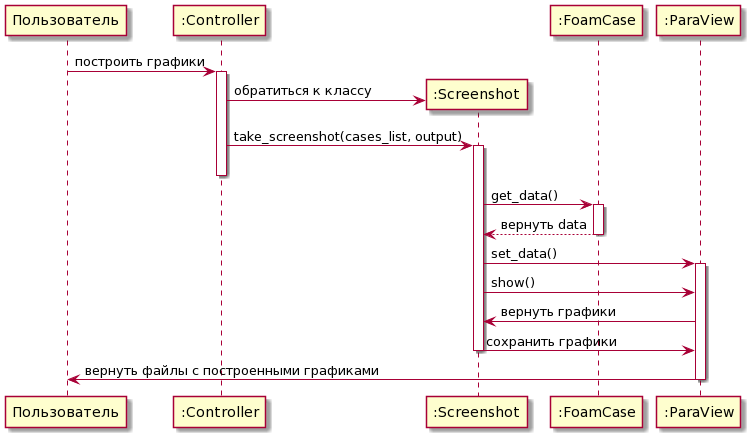
\includegraphics[width=1.1 \linewidth]{sequenceDiagram_graphs}}
\caption{Диаграмма последовательностей для прецедента <<Построение графиков примера>>}
\label{fig9}
\end{figure}

В соответствии с рисунком ~\ref{fig10} представлена диаграмма последовательностей для прецедента <<Построение графиков примера>>.

\begin{figure}[H]
\centerline{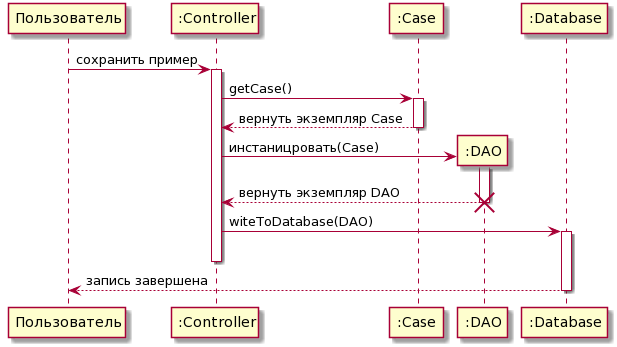
\includegraphics[width=1.1 \linewidth]{sequenceDiagram_saveToDB}}
\caption{Диаграмма последовательностей для прецедента <<Сохранение примера в базу данных>>}
\label{fig10}
\end{figure}

В соответствии с рисунком ~\ref{fig11} представлена диаграмма последовательностей для прецедента <<Добавление источника данных>>.

\begin{figure}[H]
\centerline{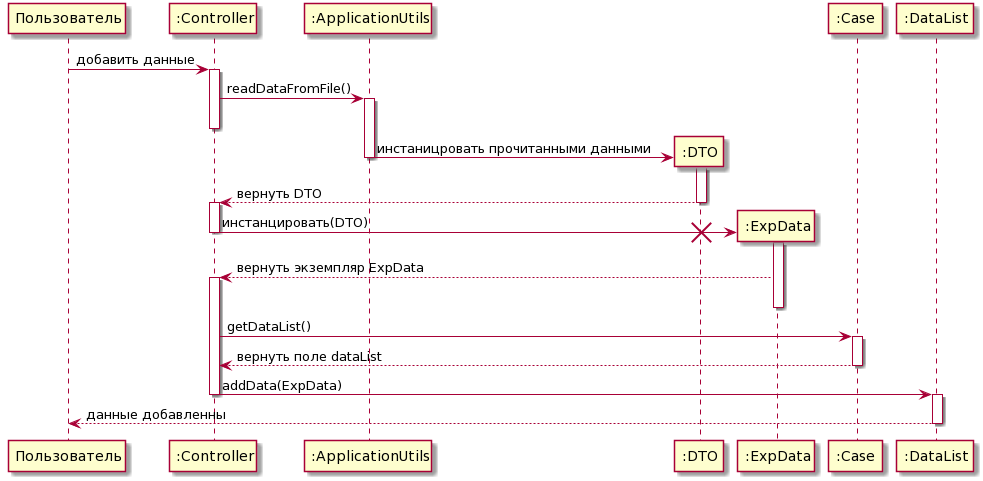
\includegraphics[width=1.1 \linewidth]{sequenceDiagram_addData}}
\caption{Диаграмма последовательностей для прецедента <<Добавление источника 
данных>>}
\label{fig11}
\end{figure}

\chapter{Выбор средств разработки}
Для хранения данных был выбран NoSQL подход. Этот выбор обусловлен теми преимуществами, которые предоставляют СУБД этого вида, а именно:
\begin{itemize}
\item Не требуется иметь строгую схему данных
\item Линейная масштабируемость
\end{itemize}

В качестве базы данных приложения была выбрана документоориентированная СУБД MongoDB, как одна из наиболее известных СУБД это вида. Рассмотрим данную базу данных и сам подход NoSQL.


\section{NoSQL}
NoSQL (с английского not only SQL, что означает не только SQL). Это обозначение широкого класса различных систем управления базами данных, появившихся в период с конца 2000-х -- начала 2010-х годов и существенно отличающихся от традиционных реляционных СУБД с доступом к данным средствами языка SQL. Применяется к системам, в которых делается попытка решить проблемы масштабируемости и доступности за счёт полного или частичного отказа от требований атомарности и согласованности данных \cite{nosqlFauler}. 

Существует несколько видов NoSQL СУБД:
\begin{itemize}
	
	\item База данных <<ключ-значение>>. Это наиболее простой вариант хранилища данных, использующий ключ для доступа к значению в рамках большой хэш-таблицы \cite{nosqlAws}. Такие СУБД применяются для хранения изображений, создания специализированных файловых систем, в качестве кэшей для объектов, а также в масштабируемых Big Data системах, включая игровые и рекламные приложения, а также проекты интернета вещей (Internet of Things, IoT). Наиболее известными представителями нереляционных СУБД типа key-value считаются Oracle NoSQL Database, Berkeley DB, MemcacheDB, Redis, Riak, Amazon DynamoDB, которые поддерживают высокую разделяемость, обеспечивая беспрецедентное горизонтальное масштабирование, недостижимое при использовании других типов БД \cite{nosqlTp}.
	
	
	\item Документоориентированные СУБД. В ней находятся данные представленные парами ключ-значение, которые сжимаются в виде полуструктурированного документа из тегированных элементов, подобно JSON, XML, BSON и другим подобным форматам \cite{nosqlAws}. Такая модель хорошо подходит для каталогов, пользовательские профилей и систем управления контентом, где каждый документ уникален и изменяется со временем \cite{nosqlTp}.  Поэтому чаще всего документные NoSQL-СУБД используются в CMS-системах, издательском деле и документальном поиске. Примеры документно-ориентированных нереляционных баз данных -- это CouchDB, Couchbase, MongoDB, eXist, Berkeley DB XML  \cite{nosqlWiki}.
	\item Колоночная база данных. Хранит информацию в виде разреженной матрицы, строки и столбцы которой используются как ключи. В мире Big Data к колоночным хранилищам относятся базы типа «семейство столбцов» (Column Family). В таких системах сами значения хранятся в столбцах (колонках), представленных в отдельных файлах. Благодаря такой модели данных можно хранить большое количество атрибутов в сжатом виде, что ускоряет выполнение запросов к базе, особенно операции поиска и агрегации данных. Наличие временных меток (timestamp) позволяет использовать такие СУБД для организации счётчиков, регистрации и обработки событий, связанных со временем: системы биржевой аналитики, IoT/IIoT-приложения, систему управления содержимым и так далее Самой известной колоночной базой данных является Google Big Table, а также основанные на ней Apache HBase и Cassandra. Также к этому типу относятся менее популярные ScyllaDB, Apache Accumulo и Hypertable.
	\item Графовая база данных. Такие хранилища представляют собой сетевую базу, которая использует узлы и рёбра для отображения и хранения данных \cite{nosqlTp}. Поскольку рёбра графа являются хранимыми, его обход не требует дополнительных вычислений (как соединение в SQL). При этом для нахождения начальной вершины обхода необходимы индексы. Обычно графовые СУБД поддерживают ACID-требования и специализированные языки запросов (Gremlin, Cypher, SPARQL, GraphQL и так далее). Такие СУБД используются в задачах, ориентированных на связи: социальные сети, выявление мошенничества, маршруты общественного транспорта, дорожные карты, сетевые топологии. Примеры графовых баз: InfoGrid, Neo4j, Amazon Neptune, OrientDB, AllegroGraph, Blazegraph, InfiniteGraph, FlockDB, Titan, ArangoDB.	
\end{itemize}

Обратимся еще раз к документоориентированной СУБД. Она включает в себя кодировку документа, хранит метаданные, связанные с хранимой информацией, что даёт возможность делать запросы на основе это информации. 
Учитывая сказанное выше и также то, что такие базы данных работают без схемы данных, делает добавление полей в JSON-документы достаточно простой задачей. 

Таким образом, имеется возможность сразу хранить некий аналог объектно-ориентированной модели, что упрощает написание соответствующих классов в программе.

\section{MongoDB} 
В качестве документоориентированный СУБД будет использована MongoDB. Ввиду популярности и простоте освоения.

MongoDB -- это база данных документов с открытым исходным кодом, построенная на горизонтально-масштабируемой архитектуре. Каждая строка в базе данных MongoDB представляет собой документ, описанный на языке форматирования JSON.
В ниже для примера представлен простой документ JSON с описанием контактной информации \cite{nosqlMongo}.
\begin{lstlisting}
{
	"name" :  "Carlos Smith",
	"title" : "Product Manager",
	"location" : "New York, NY",
	"twitter" : "@MongoDB",
	"facebook" : "@MongoDB"
}
\end{lstlisting}

JSON эффективен по многим причинам:
\begin{itemize}
	\item Это естественная форма хранения данных.
	\item Легко воспринимается людьми.
	\item Структурированная и неструктурированная информация может храниться в одном документе.
    \item Благодаря JSON, документы могут иметь неограниченную вложенность друг в друга.
    \item JSON имеет гибкую и динамическую схему, поэтому добавление или удаление полей из документа не представляет каких-либо сложностей. Возможно хранить, например, частично завершенные документы.
\end{itemize}

Также важно отметить, что структура данных находится под контролем разработчика. Это в свою очередь предоставляет возможность корректировать и переформатировать базу данных по мере развития приложения без помощи администрирования базы данных. При необходимости MongoDB может координировать и контролировать изменения в структуре документов. Поля в документе играют роль столбцов в базе данных SQL, и, как столбцы, их можно индексировать для повышения производительности поиска.

MongoDB отличным пользовательский web-интерфейс, что также является плюсом.

Из недостатков следует отметить ложащуюся на разработчика ответственность за формализацию базы данных. Недостаточный контроль может привести к путанице и лишним издержкам на больших проектах.

\section{Python}
Выбор языка должен быть обусловлен возможностью интеграции с выбранной базой данных, а также обеспечивать доступ к Paraview API. В этой связи, будет рассмотрен язык программирования Python как наиболее подходящий кандидат.

Высокоуровневый язык программирования Python является языком общего назначения с динамической строгой типизацией и автоматическим управлением памятью, ориентированный на повышение производительности разработчика, читаемости кода и его качества, а также на обеспечение переносимости написанных на нём программ. Язык является полностью объектно-ориентированным -- всё является объектами \cite{PythonYogesh}. 
Характерное отличие языка -- выделение блоков кода пробельными символами или табуляцией. Синтаксис ядра языка минималистичен, за счёт чего на практике редко возникает необходимость обращаться к документации \cite{PythonLutz}. Python -- интерпретируемый мультипарадигмальный язык программирования, который используется для различных задач \cite{PythonYogesh}. Недостатками языка являются зачастую более низкая скорость работы и более высокое потребление памяти написанных на нём программ по сравнению с аналогичным кодом, написанным на компилируемых языках, таких как Си или C++ \cite{PythonLutz}. 

Тем не менее, Python будет легко использовать при дальнейшем расширении программы. Например, для добавления веб-интерфейса приложения можно будет использовать Django и flask. Или при что-то более легковесное, например FastAPI и React.

У приложения Paraview имеется API для двух языков: Python и C++. Это сразу ограничивает выбор языка разработки. Python более современный, комфортный и гибкий, часто выступает как более удобный интерфейс для C++ библиотек. Также Python имеет интеграцию с MongoDB через библиотеку PyMongo


В качестве языка программирования для написания работы был выбран Python, так как он достаточно гибкий и удобный, а также имеет интеграцию с ParaView через библиотеку ParaView Python API и с MongoDB через библиотеку PyMongo.

Немаловажная деталь это выбор среды разработки. К этом следует также подходить внимательно, так как верно выбранная среда сильно сокращает время написания, отладки и тестирования программы. Остановимся PyCharm Community Edition от компании JetBrains. Скриншот окна программы представлен в соответствии с рисунком ~\ref{fig12}.

\begin{figure}[H]
	\centerline{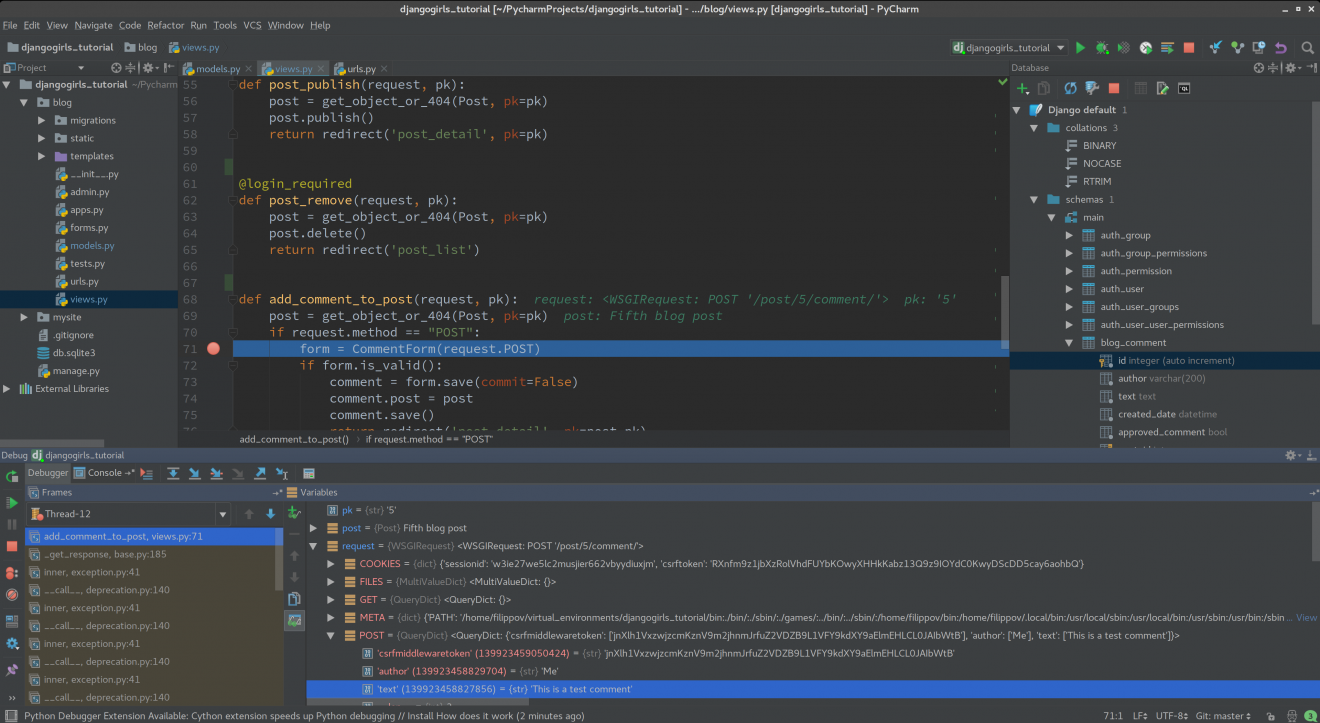
\includegraphics[width=1.1 \linewidth]{pycharm}}
	\caption{Рабочее окно программы PyCharm}
	\label{fig12}
\end{figure}

 Выбор обусловлен тем, что во-первых, данное интегрированное средство разработки доступно под операционной системой Linux \cite{IDEComp}, что необходимо для тестирования так как средствами ParaView будут считываться данные расчетов полученные от пакета программ OpenFOAM, который в свою очередь работает только под операционной системой из семейства Linux. Во-вторых, средства отладки и автозаполнения кода предоставляются из коробки, что дает возможность не тратить время на установку и налаживание работы. В-третих, в PyCharm присутствует нативная интеграция виртуальным окружением Conda, которое сильно упрощает установки ParaView Python API.
 
 Таким образом, перечисленные выше преимущества объясняют выбор конкретно этой среды разработки. 

\section{Обзор средств разработки графического интерфейса пользователя}
Также необходимо выбрать фреймворк для разработки графического интерфейса пользователя приложения. Принимая во внимание, что мы разрабатываем на Python и, учитывая, потенциальную расширяемость программы.  

\subsection{Kivy}
Kivy -- это бесплатный фреймворк Python с открытым исходным кодом для разработки мобильных приложений и другого программного обеспечения для  широкого назначения с естественным пользовательским интерфейсом. Он распространяется в соответствии с условиями лицензии MIT, что дает право использовать библиотеку бесплатного в личных и коммерческих целях. Kivy может работать на Android, iOS, Linux, macOS и Windows \cite{kivy}. 

\begin{figure}[H]
	\centerline{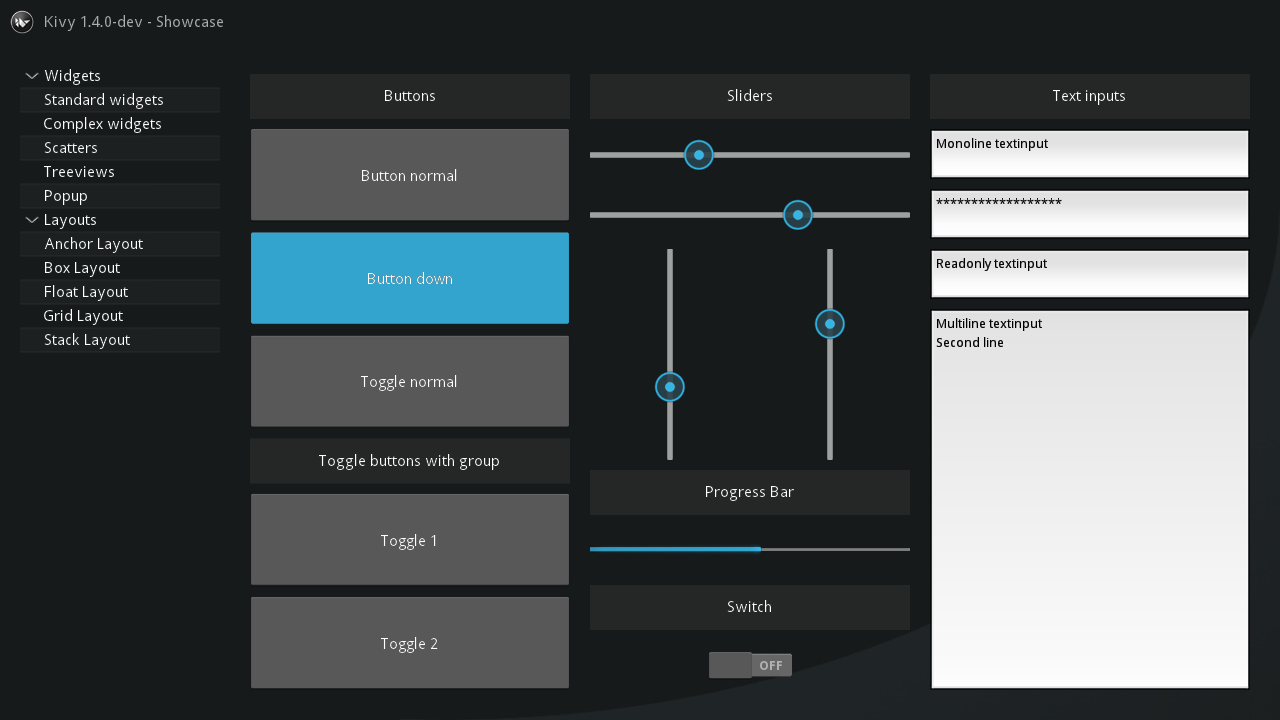
\includegraphics[width=1.1 \linewidth]{kivy}}
	\caption{Приложение Kivy}
	\label{fig13}
\end{figure}

Фреймворк содержит все элементы для создания приложения, такие как:
\begin{itemize}
\item Расширенная поддержка ввода для мыши, клавиатуры, TUIO и событий мультитач ОС.
\item Графическая библиотека, использующая только OpenGL ES 2 и основанная на Vertex Buffer Object и шейдерах.
\item Широкий выбор виджетов, поддерживающих мультитач.
\item Промежуточный язык, используемый для простой разработки пользовательских виджетов.
\end{itemize}

\subsection{TKinter}

Tkinter -- это событийно-ориентированная кросс-платформенная графическая библиотека. Она достаточно широко распространена в мире GNU/Linux и других UNIX‐подобных систем, портирована также и на Microsoft Windows. Входит в стандартную библиотеку Python и является свободным программным обеспечением.

Преимущества:
\begin{itemize}
	\item	 Краткость. Программы Python, использующие Tkinter, могут быть весьма короткими. Например, для многих используемых для создания виджетов параметров, значениям по умолчанию заданы разумные значения, что в комбинации с Python дает весьма компактный код.
	
	\item Кросс-платформенный. Tk предоставляет виджеты для Windows, Mac и большинства реализаций Unix. При это существуюет зависимость от платформы, но небольшая.
	
	\item Ядро хорошо разработано и стабильно
	
	\item Расширяемость. Существует множество расширений Tk.

\end{itemize}

Недостатки Tkinter -- скорость. Большинство вызовов Tkinter форматируются как Tcl-команда и интерпретируются c помощью Tcl. Отсюда фактические и выполняются вызовы Tkinter. Таким образом происходит последовательный вызов двух интерпретируемых языков \cite{pythonRob}.

\subsection{wxPython}
wxPython - это кроссплатформенный набор инструментов с графическим интерфейсом для языка программирования Python. Он позволяет программистам Python просто и легко создавать программы с графическим пользовательским интерфейсом. Он реализован в виде набора модулей расширения Python, которые обертывают компоненты графического интерфейса популярной кроссплатформенной библиотеки wxWidgets, написанной на C++ \cite{wxpython}.

Подобно Python и wxWidgets, wxPython является открытым исходным кодом. Также он является кроссплатформенным инструментарием. В настоящее время поддерживаемыми платформами являются Microsoft Windows, Mac OS X и macOS, а также Linux или другие unix-подобные системы с библиотеками GTK2 или GTK3.

Присутствует официальная документация, но не хватает сторонних источников и примеров использования библиотеки.

\subsection{PyQt/PySide}
PyQt — набор расширений (биндингов) графического фреймворка Qt для языка программирования Python, выполненный в виде расширения Python.

PyQt работает на всех платформах, поддерживаемых Qt: Linux и другие UNIX-подобные ОС, Mac OS X и Windows. Существует 2 версии: PyQt5, поддерживающий Qt 5, и PyQt4, поддерживающий Qt 4. PyQt распространяется под лицензиями GPL (2 и 3 версии) и коммерческой \cite{pyqt}. 

PyQt также включает в себя Qt Designer (Qt Creator) — дизайнер графического интерфейса пользователя. Программа pyuic генерирует Python код из файлов, созданных в Qt Designer. Это делает PyQt очень полезным инструментом для быстрого прототипирования. Кроме того, можно добавлять новые графические элементы управления, написанные на Python, в Qt Designer. 

Однако, для PyQt существуют ограничения связанные с лицензией GPL, поэтому был разработан PySide. PySide -- привязка языка Python к инструментарию Qt, совместимая на уровне API с PyQt. В отличие от PyQt, PySide доступна для свободного использования как в открытых, так и закрытых, в частности, коммерческих проектах, поскольку лицензирована по LGPL \cite{pyside}. 

Все представленные библиотеки имеют примерно одинаковые преимущества, но стоит выбирать наиболее зрелые и популярные. Это даст возможность в случаи необходимости легко найти решение проблем, возникающих в процессе разработки приложения. PySide кажется хорошим вариантом.

\begin{figure}[H]
	\centerline{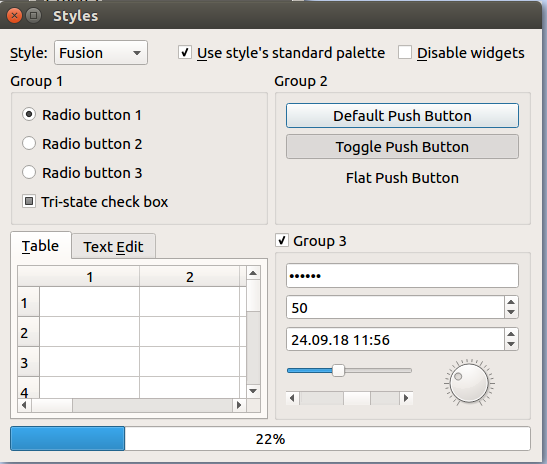
\includegraphics[scale=0.7]{pyqtscreenshot}}
	\caption{Приложение PySide}
	\label{fig14}
\end{figure}

Преимущества PySide с точки зрения выбора фреймворка:
\begin{itemize}
	\item Стабильность.
	\item Подробнейшая документация.
	\item Обилие дополнительной информации на различных форумах и сайтах.
\end{itemize}

Недостатки:
\begin{itemize}
	\item Сложность в освоении из-за большого размера.
	\item Не вся документация доступна для языка Python.
\end{itemize}

Но эти недостатки нивелируются. В частности, первый из них не имеет значения, если есть некий опыт работы и общее понимание принципов устройства фреймворка. А второй недостаток, также преодолевается опытом,подобием синтаксиса в целом и большим количеством сторонней информации в сети интернет.

Таким образом, предпочтение было отдано PySide6. 

\chapter{Разработка}


\conclusions

В данной работе кратко рассмотрен пакет программ для численного моделирования OpenFOAM, приложения для пост-процессинга ParaView. Была поставлена задача проектирования информационной системы. Выполнена первая итерация проектирования, необходимая для начала написания приложения, в частности построены UML-диаграммы прецедентов, классов, последовательностей. Также были рассмотрены существующие на данным момент решение по пост-обработки экспериментальных данных и выбраны средства разработки.

Таким образом, задачи данной работы были выполнены и, следовательно, поставленная цель была достигнута. 

% Оформляем библиографию в соответствии с ГОСТ 7.0.5
\bibliographystyle{ugost2008}
% если хотим включить все источники из библиографии даже не имеющие ссылки из текта
% \nocite{*}
% файл с библиографией
% \bibliography{biblio.bib}

\begin{thebibliography}{9}

\bibitem{OpenfoamWiki} 
   Статья OpenFOAM [Электронный ресурс] : (на 08 апреля 2020 года) // Официальный веб-сайт Wikipedia [Электронный ресурс] : [сайт]. - URL: https://ru.wikipedia.org/wiki/OpenFOAM (дата обращения 08.04.2020). - Загл с экрана - Яз. рус.
   
\bibitem{OpenfoamUserGuide} 
   Страница User guide [Электронный ресурс] : (на 08 апреля 2020 года) // Официальный веб-сайт OpenFOAM [Электронный ресурс] : [сайт]. - URL: https://cfd.direct/openfoam/user-guide (дата обращения 08.04.2020). - Загл с экрана - Яз. англ.
   
\bibitem{ParaviewAbout} 
   Страница About [Электронный ресурс] : (на 08 апреля 2020 года) // Официальный веб-сайт ParaView [Электронный ресурс] : [сайт]. - URL: https://www.paraview.org/overview (дата обращения 08.04.2020). - Загл с экрана - Яз. англ.
   
\bibitem{ParaviewWiki} 
   Статья ParaView [Электронный ресурс] : (на 09 апреля 2020 года) // Официальный веб-сайт Wikipedia [Электронный ресурс] : [сайт]. - URL: https://ru.wikipedia.org/wiki/ParaView (дата обращения 09.04.2020). - Загл с экрана - Яз. рус.
   


\bibitem{ParaviewAndPython} 
   Страница ParaView and Python [Электронный ресурс] : (на 10 апреля 2020 года) // Официальный веб-сайт ParaView [Электронный ресурс] : [сайт]. - URL: https://www.paraview.org/Wiki/ParaView\_and\_Python (дата обращения 10.04.2020). - Загл с экрана - Яз. англ.
  
\bibitem{Helyx} 
   Продукт Helyx OS [Электронный ресурс] : (на 29 марта 2020 года) // Официальный веб-сайт Helyx [Электронный ресурс] : [сайт]. - URL: https://engys.com/products/helyx-os (дата обращения 29.03.2020). - Загл с экрана - Яз. англ.
      
\bibitem{Ansa} 
   Продукт ANSA [Электронный ресурс] : (на 11 апреля 2020 года) // Официальный веб-сайт компании Beta [Электронный ресурс] : [сайт]. - URL: http://www.beta-cae.gr/ansa.html (дата обращения 11.04.2020). - Загл с экрана - Яз. англ.
   
\bibitem{CastNet} 
   Продукт CastNet [Электронный ресурс] : (на 11 апреля 2020 года) // Официальный веб-сайт компании DHCAE Tools [Электронный ресурс] : [сайт]. - URL: http://www.dhcae-tools.com/CastNet.html (дата обращения 11.04.2020). - Загл с экрана - Яз. англ.  

\bibitem{umlDistilled}
  Фаулер, М. UML. Основы, 3-е издание/ М. Фаулер -- Спб: Символ-Плюс, 2004. - 192с.
  
\bibitem{oop}
  Гамма, Э. Приемы объектно-ориентированного проектирования/ Э. Гамма, Р. Хелм, Р. Джонсон, Д. Влиссидес -- Спб: Питер, 2019. - 368 с.
  
\bibitem{pattern} 
  Паттерны проектирования. Команда [Электронный ресурс] : (на 19 апреля 2020 года) // Веб-сайт refactoring guru [Электронный ресурс] : [сайт]. - URL: https://refactoring.guru/ru/design-patterns/command (дата обращения 19.04.2020). - Загл с экрана - Яз. рус.
  
\bibitem{umlApplying}
  Ларман, К. Применение UML 2.0 и шаблонов проектирования. Практическое руководство. 3-е издание/ К. Ларман -- М: И.Д. Вильямс, 2013. - 736 с.
  
\bibitem{nosqlFauler}
     Фаулер М., Садаладж П. NoSQL. Методология разработки нереляционных баз данных / М. Фаулер -- Диалектика-Вильямс, 2020. - 192 с.
     
\bibitem{nosqlAws} 
Обзор NoSQL [Электронный ресурс] : (на 19 апреля 2020 года) // Веб-сайт Amazon Web Services [Электронный ресурс] : [сайт]. - URL: https://aws.amazon.com/ru/nosql/ (дата обращения 19.04.2021). - Загл с экрана - Яз. рус.

\bibitem{nosqlTp} 
Разбираемся в типах NoSQL СУБД [Электронный ресурс] : (на 19 апреля 2020 года) // Веб-сайт Tproger [Электронный ресурс] : [сайт]. - URL: https://tproger.ru/translations/types-of-nosql-db/ (дата обращения 19.04.2021). - Загл с экрана - Яз. рус.

\bibitem{nosqlWiki} 
NoSQL СУБД [Электронный ресурс] : (на 20 апреля 2020 года) // Веб-сайт wikipedia [Электронный ресурс] : [сайт]. - https://ru.wikipedia.org/wiki/NoSQL (дата обращения 20.04.2021). - Загл с экрана - Яз. рус.


\bibitem{nosqlMongo} 
MongoDB [Электронный ресурс] : (на 23 апреля 2020 года) // Веб-сайт mongodb [Электронный ресурс] : [сайт]. - https://www.mongodb.com/why-use-mongodb (дата обращения 23.04.2021). - Загл с экрана - Яз. англ.

\bibitem{PythonYogesh}
Yogesh R., Python: Simple though an Important Programming language [Текст]  / R. Yogesh // International Research Journal of Engineering and Technology (IRJET). – 2019. - том 06, номер 2. – С. 1856—1858.

\bibitem{PythonLutz}
Лутц, М. Программирование на Python, том 1 / М. Лутц -- СПб: Символ-Плюс, 2011. - 992 с.

\bibitem{IDEComp}
Сравнение интегрированных сред разработки [Электронный ресурс] : (на 24 апреля 2020 года) // Веб-сайт wikipedia [Электронный ресурс] : [сайт]. - https://en.wikipedia.org/wiki/Comparison\_of\_integrated\_development\_environments\#Python (дата обращения 24.04.2021). - Загл с экрана - Яз. англ.

\bibitem{kivy}
Страница о нас [Электронный ресурс] : (на 30 апреля 2020 года) // Веб-сайт фреймворка Kivy [Электронный ресурс] : [сайт]. - https://kivy.org/\#aboutus (дата обращения 30.04.2021). - Загл с экрана - Яз. англ.

\bibitem{pyqt}
PyQt. Введение [Электронный ресурс] : (на 30 апреля 2020 года) // Веб-сайт Riverbank Computing [Электронный ресурс] : [сайт]. - https://riverbankcomputing.com/software/pyqt/intro (дата обращения 30.04.2021). - Загл с экрана - Яз. англ.

\bibitem{pyside}
Qt for Python [Электронный ресурс] : (на 30 апреля 2020 года) // Веб-сайт Wiki Qt[Электронный ресурс] : [сайт]. - https://wiki.qt.io/Qt\_for\_Python/ru (дата обращения 30.04.2021). - Загл с экрана - Яз. рус.

\bibitem{pythonRob}
Robinson A. Python Programming On Win32 / A. Robinson, M. Hammond -- O'Reilly Media, 2000. - 674 с.

\bibitem{wxpython}
Overview of wxPython [Электронный ресурс] : (на 30 апреля 2020 года) // Веб-сайт wxPython [Электронный ресурс] : [сайт]. - https://www.wxpython.org/pages/overview/ (дата обращения 30.04.2021). - Загл с экрана - Яз. ангд.



\end{thebibliography}


% \Appendix % Приложения

\end{document}
